%%%%%%%%%%%%%%%%%%%%%%%%%%%%%%%%%%%%%%%%%
% Short Sectioned Assignment LaTeX Template Version 1.0 (5/5/12)
% This template has been downloaded from: http://www.LaTeXTemplates.com
% Original author:  Frits Wenneker (http://www.howtotex.com)
% License: CC BY-NC-SA 3.0 (http://creativecommons.org/licenses/by-nc-sa/3.0/)
%%%%%%%%%%%%%%%%%%%%%%%%%%%%%%%%%%%%%%%%%

%----------------------------------------------------------------------------------------
%	PACKAGES AND OTHER DOCUMENT CONFIGURATIONS
%----------------------------------------------------------------------------------------

\documentclass[paper=a4, fontsize=11pt]{scrartcl} % A4 paper and 11pt font size

% ---- Entrada y salida de texto -----

\usepackage[T1]{fontenc} % Use 8-bit encoding that has 256 glyphs
\usepackage[utf8]{inputenc}
%\usepackage{fourier} % Use the Adobe Utopia font for the document - comment this line to return to the LaTeX default

% ---- Idioma --------

\usepackage[spanish, es-tabla]{babel} % Selecciona el español para palabras introducidas automáticamente, p.ej. "septiembre" en la fecha y especifica que se use la palabra Tabla en vez de Cuadro

% ---- Otros paquetes ----

\usepackage{url} % ,href} %para incluir URLs e hipervínculos dentro del texto (aunque hay que instalar href)
\usepackage{hyperref}
\hypersetup{
	colorlinks=true,
	linkcolor=black,
	urlcolor=black,
	citecolor=black,
}
\usepackage{amsmath,amsfonts,amsthm} % Math packages
%\usepackage{graphics,graphicx, floatrow} %para incluir imágenes y notas en las imágenes
\usepackage{graphics,graphicx, float} %para incluir imágenes y colocarlas

% Para hacer tablas comlejas
%\usepackage{multirow}
%\usepackage{threeparttable}

%\usepackage{sectsty} % Allows customizing section commands
%\allsectionsfont{\centering \normalfont\scshape} % Make all sections centered, the default font and small caps

\usepackage{fancyhdr} % Custom headers and footers
\pagestyle{fancyplain} % Makes all pages in the document conform to the custom headers and footers
\fancyhead{} % No page header - if you want one, create it in the same way as the footers below
\fancyfoot[L]{} % Empty left footer
\fancyfoot[C]{} % Empty center footer
\fancyfoot[R]{\thepage} % Page numbering for right footer
\renewcommand{\headrulewidth}{0pt} % Remove header underlines
\renewcommand{\footrulewidth}{0pt} % Remove footer underlines
\setlength{\headheight}{13.6pt} % Customize the height of the header

\numberwithin{equation}{section} % Number equations within sections (i.e. 1.1, 1.2, 2.1, 2.2 instead of 1, 2, 3, 4)
\numberwithin{figure}{section} % Number figures within sections (i.e. 1.1, 1.2, 2.1, 2.2 instead of 1, 2, 3, 4)
\numberwithin{table}{section} % Number tables within sections (i.e. 1.1, 1.2, 2.1, 2.2 instead of 1, 2, 3, 4)

\setlength\parindent{0pt} % Removes all indentation from paragraphs - comment this line for an assignment with lots of text

\newcommand{\horrule}[1]{\rule{\linewidth}{#1}} % Create horizontal rule command with 1 argument of height
\usepackage{booktabs}

\usepackage{listings}
\usepackage{color}
\usepackage{xcolor}
\lstdefinestyle{customc}{
	belowcaptionskip=1\baselineskip,
	breaklines=true,
	frame=L,
	xleftmargin=\parindent,
	language=C,
	showstringspaces=false,
	basicstyle=\footnotesize\ttfamily,
	keywordstyle=\bfseries\color{green!40!black},
	commentstyle=\itshape\color{purple!40!black},
	identifierstyle=\color{blue},
	stringstyle=\color{orange},
}

\lstset{escapechar=@,style=customc}

\title{	
	\normalfont \normalsize 
	\textsc{\textbf{Visión por Computador} \\ Grado en Ingeniería Informática \\ Universidad de Granada \\
	Curso 2017-2018} \\ [25pt] % Your university, school and/or department name(s)
	\horrule{0.5pt} \\[0.4cm] % Thin top horizontal rule
	\huge Trabajo 3. \\
	\huge Indexación y Recuperación de imágenes.
	\\ % The assignment title
	\horrule{2pt} \\[0.5cm] % Thick bottom horizontal rule
}

\author{Alberto Armijo  \\
\href{mailto:armijoalb@correo.ugr.es}{armijoalb@correo.ugr.es}} % Nombre y apellidos
\date{\normalsize\today} % Incluye la fecha actual

%----------------------------------------------------------------------------------------
% DOCUMENTO
%----------------------------------------------------------------------------------------

\begin{document}
	
	\maketitle % Muestra el Título
	
	\newpage %inserta un salto de página
	
	\tableofcontents % para generar el índice de contenidos
	
	\listoffigures % para generar índice de imágenes.
	
	\newpage
	
	\section[Ejercicio 1]{Emparejamiento de descriptores.}
	Para este primer ejercicio, utilizaremos las funciones de la práctica anterior \textbf{correspondencias2NN()} para calcular las correspondencias entre dos imágenes, también se utilizará la función \textbf{calculateDescriptors()}; para esta función se ha añadido un parámetro llamado mask con el cuál especificamos a la función de OpenCV \textbf{detectAndCompute()} la zona de la imagen para la cuál queremos calcular los descriptores.
	
	\vspace{0.06in}
	Para la creación de la máscara, se ha creado una función, llamada \textbf{createMak()}, la cuál toma como parámetros la imagen para la que se crea la máscara y las coordenadas de los puntos con los que se creará la máscara. Para crear la máscara, utilizaremos una matriz inicializada a 0, después, crearemos un polígono con los puntos que le hemos pasado a la función (utilizaremos la función \textbf{cv2.approxPollyPD}). Tras esto, introduciremos este polígono dentro de la máscara con la función \textbf{cv2.fillConvexPoly()}, hay que especificar que el color del polígono debe ser blanco, (255,255,255) si utilizamos RGB. Por último, tenemos que transformar esta máscara a blanco y negro (se puede hacer con la función \textbf{cv2.cvtColor()} ).
	
	\vspace{0.06in}
	Para tener diferentes máscaras para los diferentes ejemplos, se han creado las siguientes máscaras:
	
	\begin{figure}[H]
		\centering
		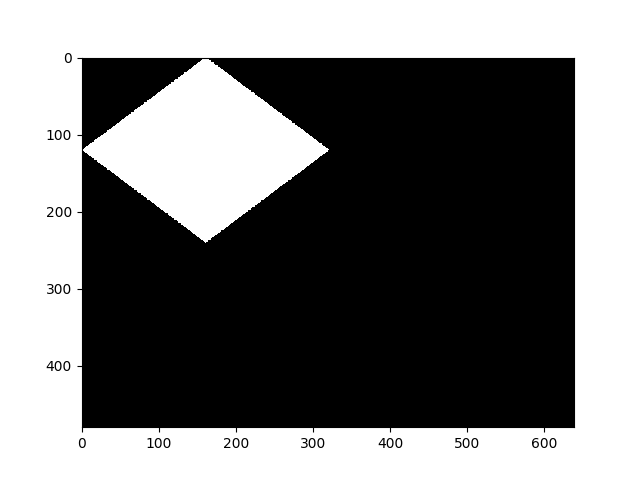
\includegraphics[scale=0.4]{./imagenes/mask1.png}
		\caption{Máscara 1}
		\label{fig:mask1}
	\end{figure}
	
	\begin{figure}[H]
		\centering
		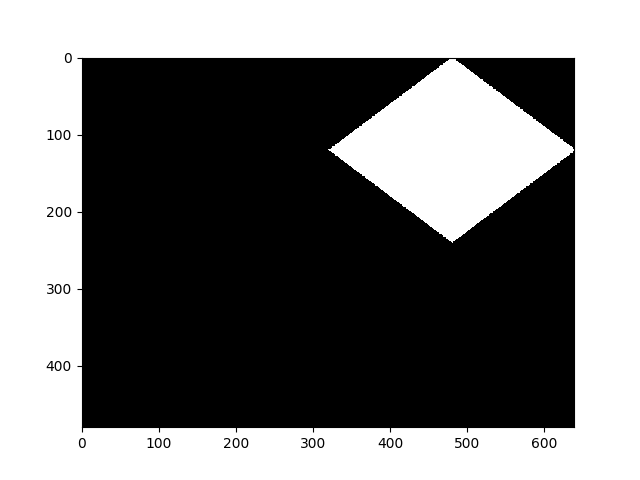
\includegraphics[scale=0.4]{./imagenes/mask2.png}
		\caption{Máscara 2}
		\label{fig:mask2}
	\end{figure}
	
	\begin{figure}[H]
		\centering
		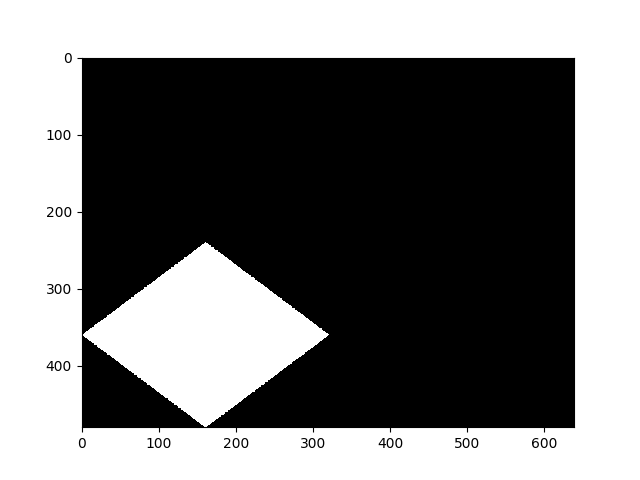
\includegraphics[scale=0.4]{./imagenes/mask3.png}
		\caption{Máscara 3}
		\label{fig:mask3}
	\end{figure}
	
	\begin{figure}[H]
		\centering
		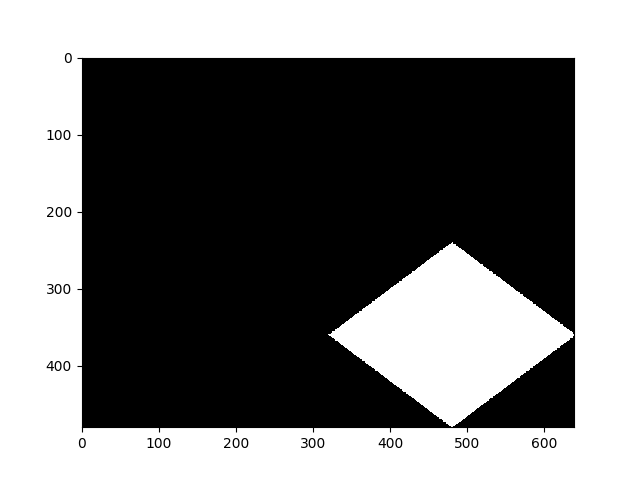
\includegraphics[scale=0.4]{./imagenes/mask4.png}
		\caption{Máscara 4}
		\label{fig:mask4}
	\end{figure}
	
	\begin{figure}[H]
		\centering
		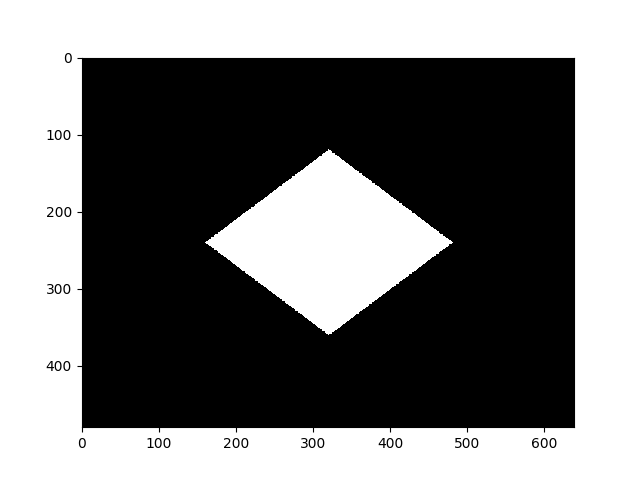
\includegraphics[scale=0.4]{./imagenes/mask5.png}
		\caption{Máscara 5}
		\label{fig:mask5}
	\end{figure}

	\vspace{0.06in}
	Ahora, utilizaremos la función \textbf{calculateCorrespondenciasWithMask()}, esta función calcula las correspondencias entre las dos imágenes que se le pasan como parámetros, pero a la primera sólo se calculan los descriptores que se encuentren dentro de la máscara. Una vez tiene los descriptores calculados, se muestran las correspondencias entre las imágenes.
	
	\vspace{0.06in}
	Para este ejercicio se han incluido dos ejemplos, formados por las parejas (128.png,130.png) y (229.png,232.png). Los resultados obtenidos son los siguientes.
	
	\vspace{0.06in}
	
	\begin{figure}[H]
		\centering
		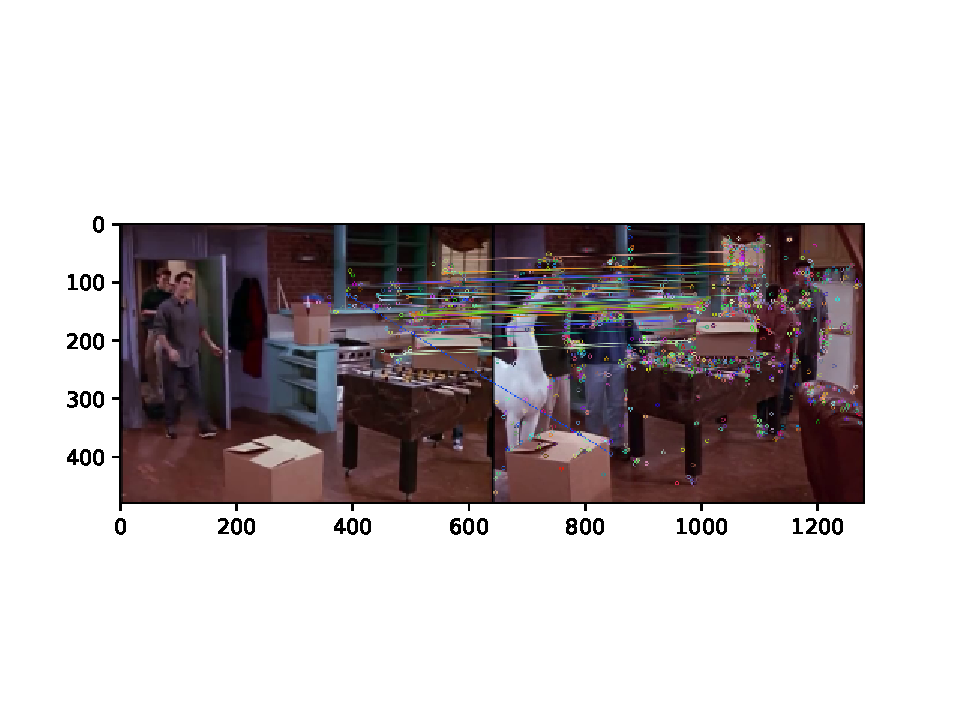
\includegraphics[scale=0.75]{./imagenes/eje1_1.pdf}
		\caption{Correspondencias 128.png y 130.png}
		\label{fig:ejer1_1}
	\end{figure}

	\begin{figure}[H]
		\centering
		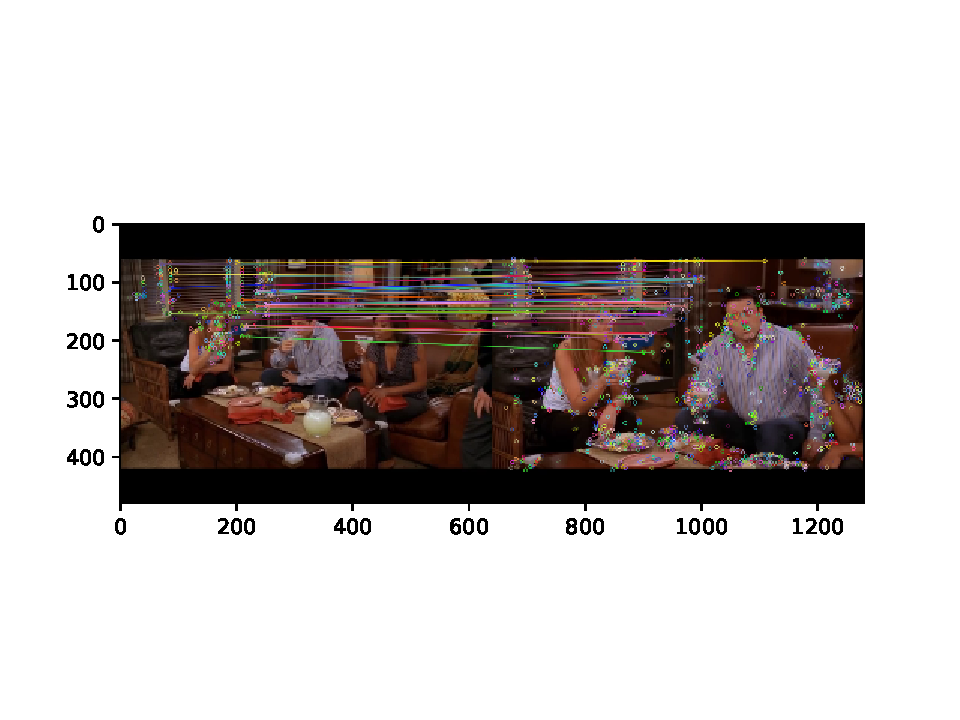
\includegraphics[scale=0.8]{./imagenes/eje1_2.pdf}
		\caption{Correspondencias 229.png y 232.png}
		\label{fig:ejer1_2}
	\end{figure}

	\vspace{0.06in}
	Como se puede ver en la imagen de las correspondencias, la mayoría de de las correspondencias son correctas, pero existen algunos errores. Esto puede ser un problema ya que para la recuperación de imágenes necesitaremos obtener características similares en ambas imágenes, y si utilizamos los descriptores como característica de la imágenes, posiblemente se obtengamos imágenes que no tienen relación con la original pero que tiene descriptores parecidos a la original.
	
	\section[Ejercicio 2]{Visualización del vocabulario.}
	Para el ejercicio 2, debemos de calcular los 20 parches más cercanos a una palabra, para ello, debemos calcular que descriptores pertenecen a la palabra y una vez que hemos obtenido los descriptores, calcularemos la distancia que hay entre ellos y la palabra visual.
	
	\vspace{0.06in}
	Para calcular los descriptores que pertenecen a la palabra visual (cluster), se ha creado la función \textbf{obtainDescriptorsPerWord}. Esta función tiene como parámetros el índice de la palabra, los descriptores y las etiquetas; lo que debemos hacer es mirar si el índice de la palabra es igual a la etiqueta correspondiente al descriptor.
	
	\vspace{0.06in}
	Ahora pasaremos a calcular la distancia entre la palabra visual y los descriptores, para ello se ha creado la función \textbf{calculateNearestDescriptors}. Esta función toma como parámetros los descriptores y la palabra. Para calcular la distancia entre los descriptores y la palabra, utilizaremos la distancia euclídea; para calcularla, utilizaremos la función \textbf{cv2.norm()} especificando su parámetro \textit{code=cv2.NORM\_L2}. Una vez hemos calculado todas las distancias, ordenaremos el vector de distancias y nos quedaremos con las 20 primeras.
	
	\vspace{0.06in}
	Además de hacer esto, dentro de esta función se calcula la varianza que hay dentro del cluster, con esto obtenemos un medida de dispersión de los clusters (palabras visuales) que después nos servirán para saber que clusters tienen un conjunto de parches más uniformes y cuáles no. Esto nos servirá a la hora de elegir ejemplos más adelante. Para calcular la varianza, utilizaremos los 10 primeros descriptores y la función \textbf{np.var()}.
	
	\vspace{0.06in}
	Por último, calcularemos los parches correspondientes, esto se hace en la función \textbf{calculateNearestPatches()} que toma como parámetros los parches y los descriptores obtenidos de la función anterior. Lo único que se hace en esta función es devolver los parches correspondientes a los índices de los descriptores que hemos calculado.
	
	\vspace{0.06in}
	Todo este proceso viene incluido dentro de la función \textbf{calculateVarianceAndBestPatchesWord()} esta toma como parámetros el índice de la palabra visual, el vocabulario, los descriptores, las etiquetas de los descriptores y los parches. También está la función \textbf{calculateVarianceAndBestPatches()}; esta realiza la misma función que la anterior pero para todas las palabras del vocabulario; esta se ha utilizado unicamente para obtener todas la varianzas y obtener los ejemplos (en el código está comentada).
	
	\vspace{0.06in}
	Para elegir ejemplos, se han tomado dos palabras que tienen poca dispersión, estas son la 931 y la 899; como tercer ejemplo se ha elegido la palabra que más dispersión tiene, la 4054. Los resultados obtenidos son los siguientes:
	
	\begin{figure}[H]
		\centering
		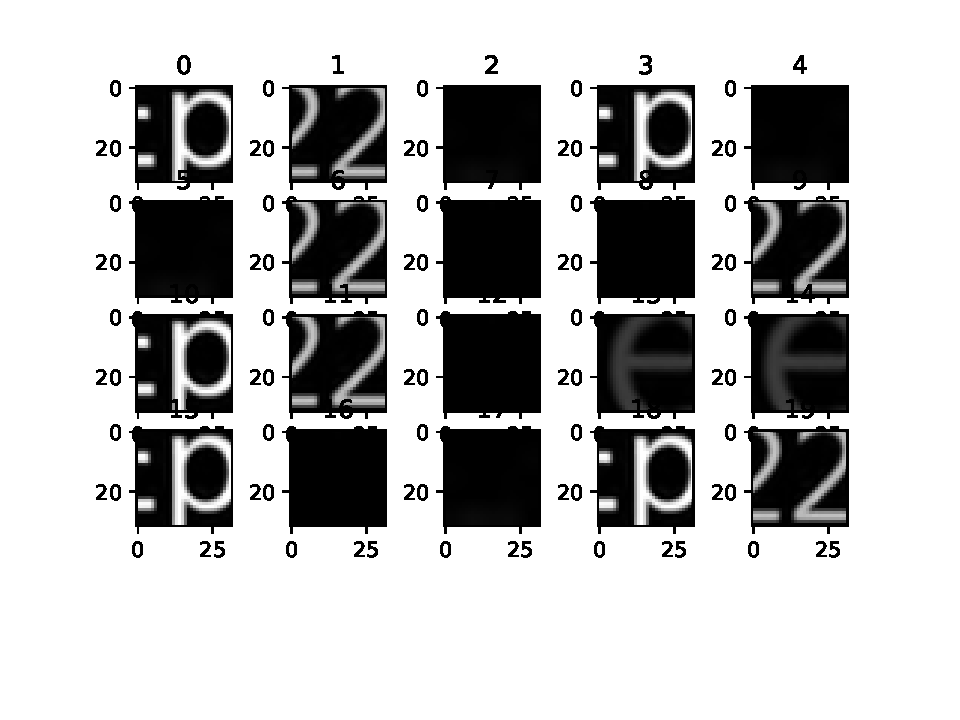
\includegraphics[scale=0.6]{./imagenes/eje2_1.pdf}
		\caption{Parches ejemplo 1}
		\label{fig:eje2_1}
	\end{figure}

	\begin{figure}[H]
		\centering
		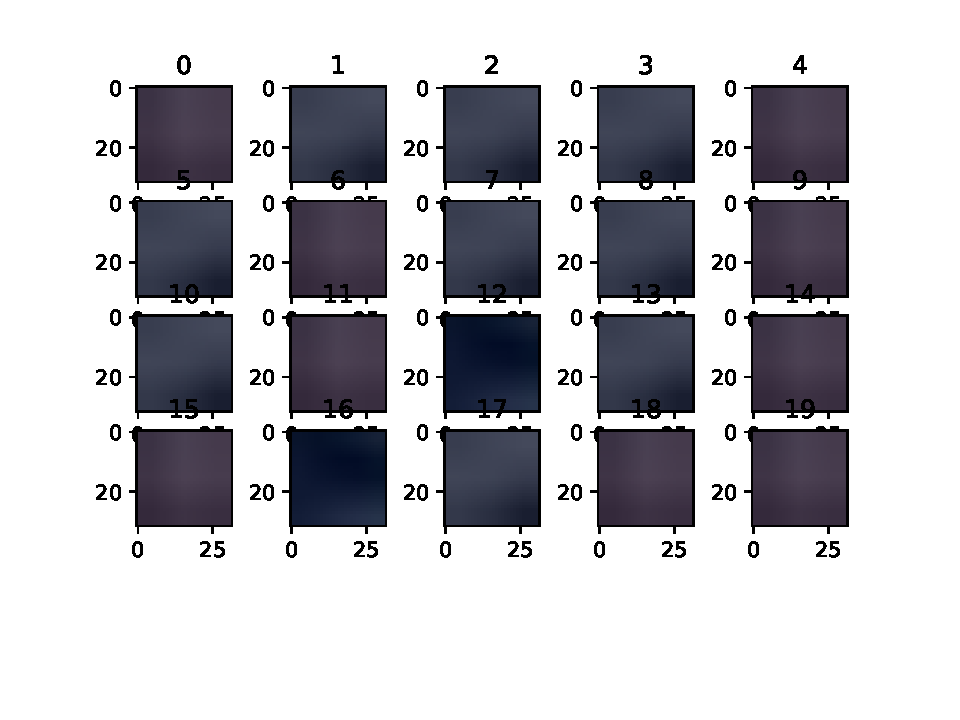
\includegraphics[scale=0.6]{./imagenes/eje2_2.pdf}
		\caption{Parches ejemplo 2}
		\label{fig:eje2_2}
	\end{figure}

	\vspace{0.06in}
	Como se puede ver en el primer ejemplo todos los parches corresponden con la zona que representa a imágenes que contiene la palabra episodio 22x.
	
	\vspace{0.06in}
	Para el segundo ejemplo podemos ver que tampoco hay mucha diferencia entre los parches, cambia el color y la intensidad de este, pero todos son más claros en el centro de la imagen.
	
	\vspace{0.06in}
	En estos dos ejemplos se cumple lo que se menciona en teoría, y es que los parches que pertenecen a una palabra deben ser muy parecidos entre ellos (si se han obtenido buenos clusters).
	
	\begin{figure}[H]
		\centering
		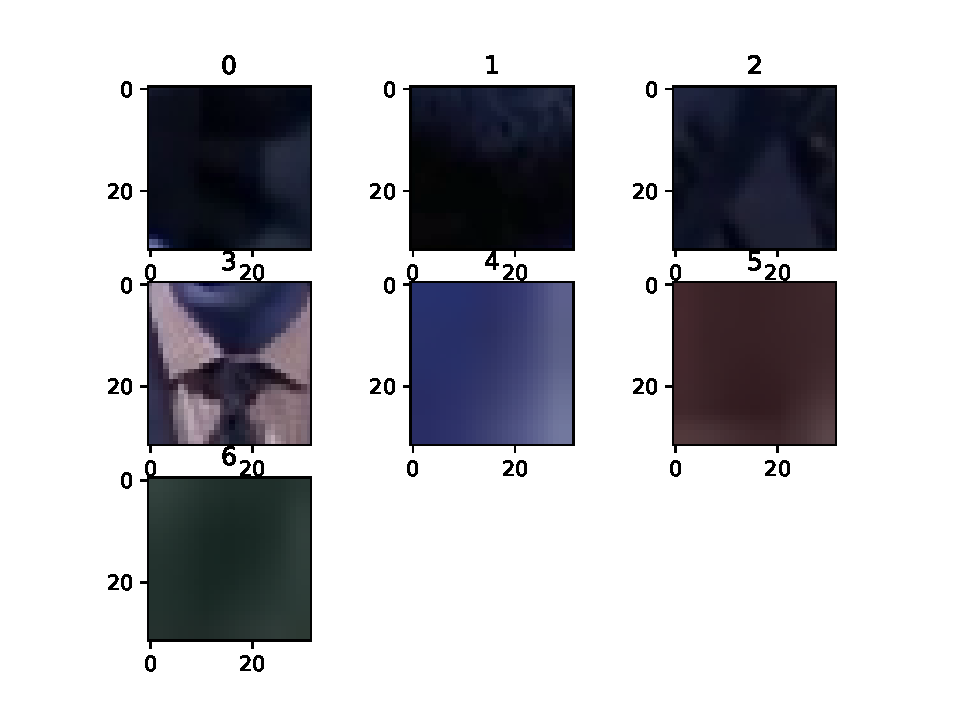
\includegraphics[scale=0.6]{./imagenes/eje2_3.pdf}
		\caption{Parches ejemplo 3.}
		\label{fig:eje2_3}
	\end{figure}

	\vspace{0.06in}
	En este tercer ejemplo, podemos ver que no hay correspondencia entre ninguna de la imágenes, y que ni siquiera hay 20 parches. Esto se debe a que el algoritmo de k-medias necesita hacer 5000 clusters por defecto y puede ocurrir que aquellas imágenes que no pueda clasificar en otros clusters la mete en un cluster aunque no se parezca, como es el caso.
	
	\section[Ejercicio 3]{Recuperación de imágenes.}
	Para el tercer ejercicio, tendremos que crear un índice invertido y calcular la bolsa de palabras de cada imagen para poder después obtener imágenes semejantes a una que se pasa como parámetro.
	
	\vspace{0.06in}
	Lo primero que debemos hacer para crear el índice invertido y el modelo de bolsa de palabras es calcular los votos para cada imagen que hay en el directorio \textit{/imágenes}, esto se hace en la función \textbf{calculateVotes()}. Para cada una de las imágenes, debemos calcular sus descriptores y normalizarlos, tras esto multiplicaremos el vocabulario de 5000 palabras por el vector de descriptores normalizado. Una vez hemos hecho esto, podremos calcular los votos que cada descriptor de la imagen, para ello recorreremos las columnas de la matriz anteriormente creada y por cada columna nos quedaremos con el índice (fila e índice de la palabra) del elemento con valor más alto. Por último, solo nos queda quedarnos con los votos que nos interesa, esto puede hacerse quedándose con las \textit{k} palabras más votadas, o bien escogiendo todas las palabras que tengan un número de votos diferente de 0.
	
	\vspace{0.06in}
	Una vez hemos obtenido las palabras más votadas en la imagen como la bolsa de palabras de la imagen (histograma de votos de la imagen), meteremos el nombre de la imagen en todos los índice del fichero invertido en los cuales tiene votos; por otro lado, guardaremos el histograma de la imagen junto con el nombre de la imagen en una estructura que guarda el modelo de palabras de todas las imágenes que se han usado. Este proceso se realiza en la función \textbf{createInvertedIndex()}
	
	\vspace{0.06in}
	Ahora tenemos que crear la segunda parte de este ejercicio, la cuál trata de obtener las imágenes semejantes a una imagen pasada.
	
	\vspace{0.06in}
	Para esto, se ha creado la función \textbf{calcualteSimilarImages()}, la cual recibe como parámetros la imagen-pregunta, el índice invertido, el modelo de bolsa de palabras y el vocabulario. Lo primero que debemos hacer es calcular las imágenes que se pueden comparar con la imagen-preguntan, esto se realiza en la función \textbf{obtainImagesFromQueryImage()}. Dentro de esa función, se calculan las palabras por las que vota la imagen-pregunta, una vez hecho esto, se extrae por cada palabra votada las imágenes en las que aparece del fichero invertido y devolvemos el conjunto de imágenes.
	Tras esto obtendremos el histograma de estas imágenes.
	
	\vspace{0.06in}
	Lo siguiente que debemos hacer el calcular qué imágenes son más semejantes a la imagen-pregunta, para ello, calcularemos el producto escalar normalizado entre la bolsa de palabra de la imagen-pregunta y cada una de las bolsas de palabras de las imágenes que hemos calculado antes. Por último, ordenamos las imágenes según el valor de la semejanza obtenido de mayor a menor y devolvemos las 5 mejores.
	
	\vspace{0.06in}
	Los resultados obtenidos son los siguientes:
	\begin{figure}[H]
		\centering
		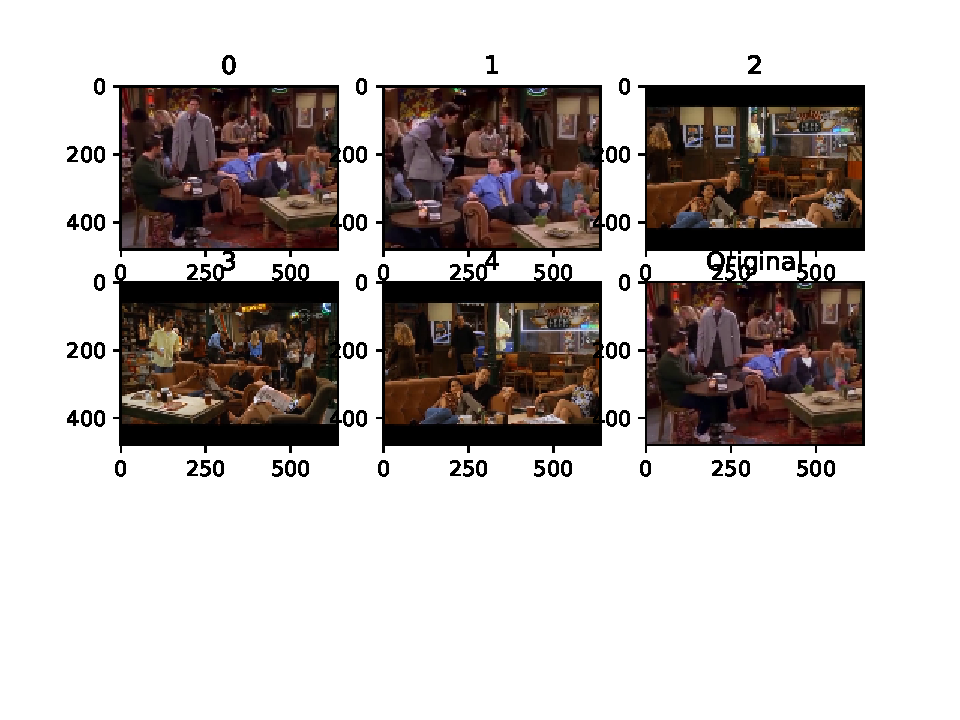
\includegraphics[scale=0.6]{./imagenes/eje3_1.pdf}
		\caption{Imágenes similares primer ejemplo.}
		\label{fig:eje3_1}
	\end{figure}
	
	\vspace{0.06in}
	Para este ejemplo podemos ver que todas las imágenes relacionadas están en la cafetería sentados en el sofá, por lo que se obtienen buenos resultados.

	\begin{figure}[H]
		\centering
		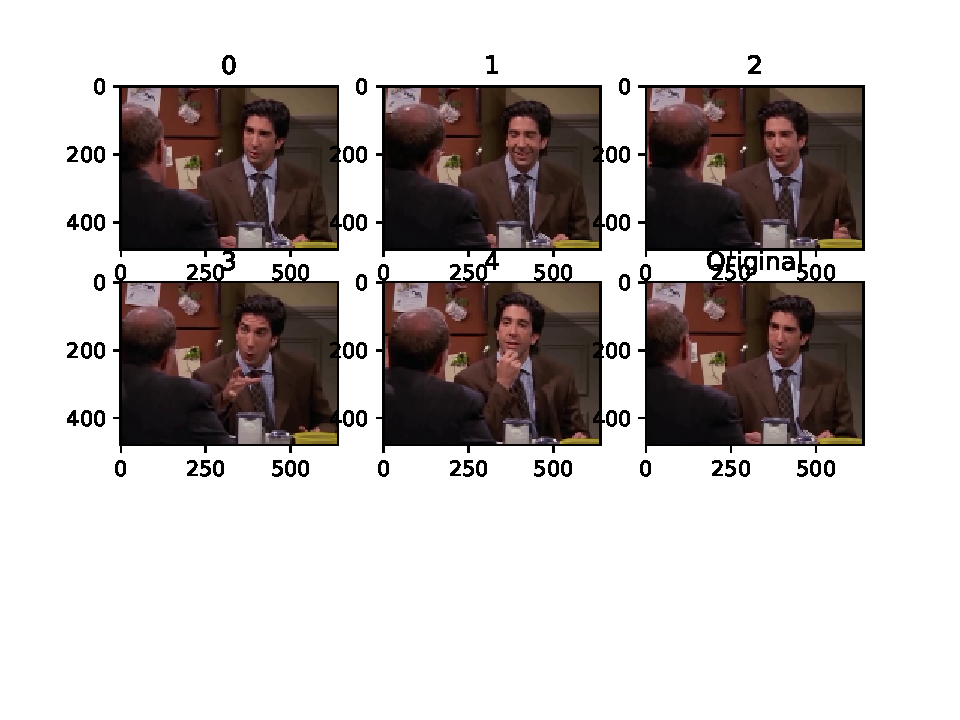
\includegraphics[scale=0.6]{./imagenes/eje3_2.pdf}
		\caption{Imágenes similares segundo ejemplo.}
		\label{fig:eje3_2}
	\end{figure}
	
	\vspace{0.06in}
	Para este segundo ejemplo los resultados también son satisfactorio ya que obtiene imágenes de la misma escena, lo único que cambia es la posición y la cara del personaje.

	\begin{figure}[H]
		\centering
		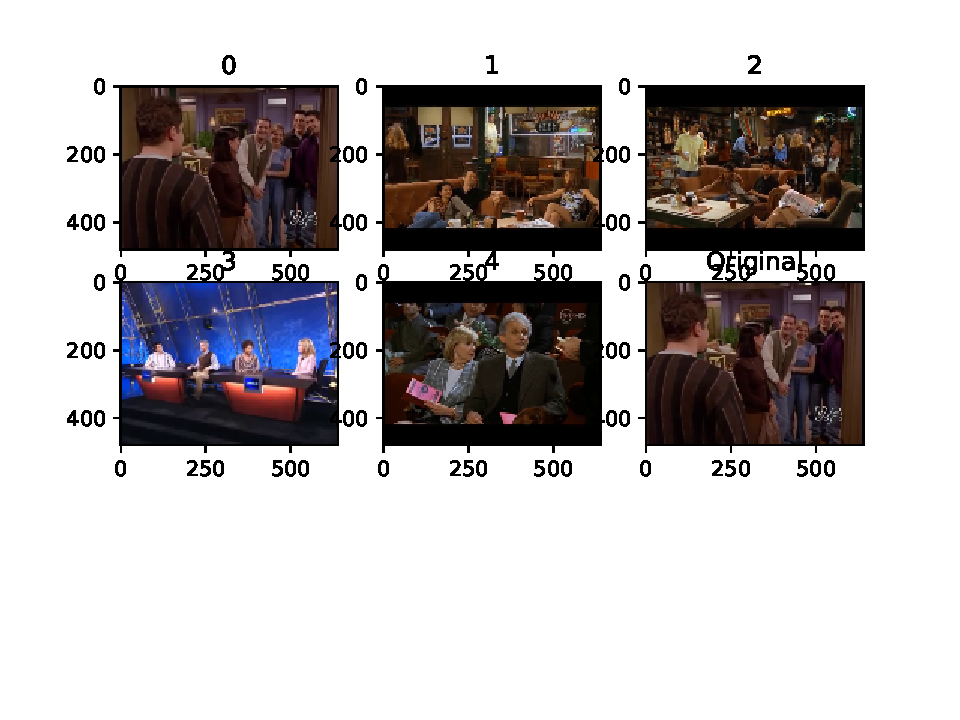
\includegraphics[scale=0.6]{./imagenes/eje3_3.pdf}
		\caption{Imágenes similares tercer ejemplo.}
		\label{fig:eje3_3}
	\end{figure}

	\vspace{0.06in}
	Para este tercer ejemplo, podemos ver que el modelo de bolsa de palabras falla, dado que en las imágenes 2 y 3 al menos aparecen varios de los personajes que aparecen en la imagen original. Sin embargo,  las últimas dos imágenes no tienen ninguna relación con la original. Esto a podido ocurrir debido a que para esta imagen no haya suficientes ejemplos parecidos dentro del conjunto de entrenamiento y por lo tanto no haya votado por palabras adecuadamente.
	
\end{document}